\documentclass[twocolumn,twoside]{article}
\usepackage[english,spanish]{babel}
\usepackage{indentfirst}
\usepackage{anysize} % Soporte para el comando \marginsize
\marginsize{2.0cm}{2.0cm}{1cm}{1cm}
%\marginsize{2,5cm}{1,8cm}{2.4cm}{1,7cm}
\usepackage[psamsfonts]{amssymb}
\usepackage{amssymb}

\usepackage{siunitx}
\sisetup{output-exponent-marker=\ensuremath{\mathrm{e}}}
\usepackage{amsfonts}
\usepackage{amsmath}
\usepackage{amsthm}
\usepackage{placeins}
\usepackage{float}
\usepackage{graphicx}
\usepackage{varioref}
\usepackage{bm}
\usepackage{enumerate} 
\usepackage{enumitem}
%\usepackage{wrapfig}
\usepackage{ragged2e,tabularx,makecell}
\renewcommand{\thepage}{}
\columnsep=7mm

%%%%%%%%%%%%%%%%%%%%%%%%%%%%%%%%%%%%%%%%
\newtheorem{definicion}{Definici\'on}[section]
\newtheorem{teorema}{Teorema}[section]
\newtheorem{prueba}{Prueba}[section]
\newtheorem{prueba*}{Prueba}[section]
\newtheorem{corolario}{Corolario}[section]
\newtheorem{observacion}{Observaci\'on}[section]
\newtheorem{lema}{Lema}[section]
\newtheorem{ejemplo}{Ejemplo}[section]
\newtheorem{solucion*}{Soluci\'on}[section]
\newtheorem{algoritmo}{Algoritmo}[section]
\newtheorem{proposicion}{Proposici\'on}[section]

\linespread{1.4} \sloppy

\newcommand{\R}{\mathbf{R}}
\newcommand{\N}{\mathbf{N}}
\newcommand{\C}{\mathbb{C}}
\newcommand{\Lr}{\mathcal{L}}
\newcommand{\fc}{\displaystyle\frac}
\newcommand{\ds}{\displaystyle}

\DeclareMathOperator{\Dom}{Dom}

%%%%%%%%%%%%%%%%%%%%%%%%%%%%%%%%%%%%%%%%

\renewcommand{\thefootnote}{\fnsymbol{footnote}}

%\setlist[enumerate]{parsep=\smallskipamount} % define el espacio entre parrafos
\begin{document}
\begin{center}
 {\Large \textbf{Aplicaci\'on de la factorizaci\'on QR usando transformaciones de Householder en m\'inimos cuadrados para un an\'alisis 
 de la pobreza en el Per\'u}}
\end{center}
\begin{center}
 Ayrton Fabio Coronado Huam\'an $^1$, Guillermo Joel Borjas C\'ordova $^2$,
 Israel Danilo Blas Salas $^3$, Tom\'as Garc\'ia Sifuentes $^4$ \vskip12pt
{\it Facultad de Ciencias $1$, Universidad Nacional de Ingenier\'{\i}a $1$, e-mail: \\
Facultad de Ciencias $2$, Universidad Nacional de Ingenier\'{\i}a $2$, e-mail:  }
\end{center}

\section{Introducc\'ion}

En este proyecto nos dedicaremos a construir un algoritmo eficiente, en t\'erminos de
tiempo de ejecuci\'on, del m\'etodo matem\'atico "Transformaci\'on de Householder", el cual
nos permite obtener un tipo de descomposici\'on de matrices llamado "Descomposici\'on QR".
Esto nos servir\'a en la resoluci\'on de un sistema de ecuaciones proveniente del ajuste de
una curva utilizando la t\'ecnica de m\'inimos cuadrados donde intervienen una variable 
dependiente y una independiente, y en la cual la relaci\'on entre ellas se aproxima por medio
de una l\'inea recta, todo esto con la finalidad de poder aplicarse a una situaci\'on 
particular en el campo de la econom\'ia, m\'as concretamente, para hacer un an\'alisis de la 
pobreza en el Per\'u y de esta manera hacer predicciones o pron\'osticos que nos ayudar\'an a 
tener un mejor entendimiento de este problema.\\
Con el fin de llevar a cabo este proyecto, se emplear\'an los datos tomados de una muestra real, 
extra\'idos de un informe hecha por el INEI de pobreza, pobreza extrema y el coeficiente de
Gini (indicador de la desigualdad econ\'omica en una poblaci\'on) en los a\~nos 2015 - 2016 de las
principales regiones del Per\'u.\\
Muchos autores que han hecho estudios sobre
modelos de regresi\'on, entre los que se pueden
citar a: Anderson, D. R., Sweeney, D. J., \& Williams,
T. A. (2001), Devore, J. L. (2005), Evans, M., \&
Rosenthal, J. S. (2005), Freund, J. E., \& Simon,
G. A. (1994), Levin, R. I., \& Rubin, D. S. (2004)
y Miller, I. (2000); coinciden en que siempre que
se analizan datos observados o recopilados para 
llegar a una funci\'on o ecuaci\'on matem\'atica que
describa la relaci\'on entre las variables por medio de
una regresi\'on, se deben enfrentar tres problemas:\\
1. Decidir qu\'e clase de curva muestran los puntos
y por tanto qu\'e clase de ecuaci\'on se debe usar.\\
2. Encontrar la ecuaci\'on particular que mejor se
ajuste a los datos.\\
3. Demostrar que la ecuaci\'on particular encontrada
cumple con ciertos aspectos referentes a los m\'eritos 
de \'esta para hacer pron\'osticos.\\
Para decidir qu\'e clase de funci\'on podr\'ia ajustarse
a la curva, debe hacerse una gr\'afica de dispersi\'on
de los datos observados. Si en dicha gr\'afica se aprecia 
que los puntos se distribuyen alrededor de una recta, se 
procede a realizar un an\'alisis de regresi\'on lineal.

\section{Conceptos Previos}
\subsection{SISTEMAS LINEALES DE ECUACIONES SOBREDETERMINADOS}
\boldmath
El problema lineal de m\'inimos cuadrados se acerca a la optimizaci\'on
si se encuentra un vector $x$ que en alg\'un sentido da la mejor (aunque no la perfecta)
aproximaci\'on entre  $Ax$ y $b$.\\
Consid\'erese un sistema de $m$ ecuaciones con $n$ inc\'ognitas escrito en la forma 
\begin{center}
 $Ax=b$ \hspace{3cm}     \textbf{(II.1)}
\end{center}
Aqu\'i, $A$ es de $m\times n$, $x$ es de $n\times 1$ y $b$ es de $m\times 1$. Supondremos que el rango de $A$ es
$n$, de lo que resulta que $m\geq n$. Si $m> n$, se dice que el sistema lineal de ecuaciones es
sobredeterminado. Los sistemas sobredeterminados son generalmente no compatibles.

\subsection{EL VECTOR RESIDUAL Y EL PROBLEMA DE LOS M\'INIMOS CUADRADOS}

Por lo general, el sistema \textbf{(II.1)} no tiene soluci\'on debido a que b no pertenece al
subespacio de $R^n$ de dimensi\'on $n$, generado por las columnas de $A$. Es frecuente en tales
casos que se requiera encontrar un $x$ tal que $b$ est\'e cerca de $A x$, es decir que minimice
una norma del vector residual $r = b-A x$. El primer problema ser\'a determinar el sentido
de cercan\'ia, es decir la norma que mide la diferencia entre $b$ y $A x$. La interpretaci\'on
y la naturaleza de la soluci\'on de este problema var\'ia dependiendo de la norma que se
use. La norma m\'as com\'unmente usada es la norma euclidiana, la norma $l_2$ . Entonces, la
soluci\'on en m\'inimos cuadrados de \textbf{(II.1)} es el vector $x$ que hace de $||r||_2 = ||b - A x||_2$
un m\'inimo
\begin{center}
  $\min\limits_{x\in R^n}||b - A x||_2^2$, \hspace{2.5cm} (II.2)
\end{center}


Dado que las normas no pueden ser negativas, minimizar una norma es equivalente a
minimizar su cuadrado; hableremos entonces libremente de normas cuadradas y no. Seg\'un
lo que se ha supuesto acerca del rango de $A$, la soluci\'on $x$ ser\'a \'unica.\\
Veremos que el problema de m\'inimos cuadrados se puede resolver transformando la
matriz $A$ y resolviendo un sistema compatible a ella relacionado. Al contrario, minimizar
la norma $l_1$ o la norma $l_\infty$ es equivalente a un problema de programaci\'on lineal no
diferenciable, cuya soluci\'on necesita una t\'ecnica de iteraci\'on.\\
Es \'util pensar en el problema de los m\'inimos cudrados en t\'erminos de los subespa-
cios definidos por la matriz $A$. El subespacio rango de $A$, rango($A$), consiste en todos
los vectores $m$-dimensionales que son combinaciones lineales de las columnas de $A$ y el
subespacio complementario, el subespacio nulo de $A^t$ , $nulo(A)$, contiene todos los vectores
$m$-dimensionales que son $z$-ortogonales a las columnas de $A$, es decir tales que $A^t z = 0$.
Si $r$ denota el rango de la matriz $A$, entonces $r$ es la dimensi\'on del subespacio rango de
$A$ y $(m - r)$ es la dimensi\'on del subespacio nulo de $A^t$ .
Dada una matriz no nula $A$, cualquier vector $m$-dimensional $c$ se puede expresar
como la suma de un vector $c_R$ en el rango de $A$, $c_R \in rango(A)$, y de un vector $c_N$ en el
espacio nulo de $A^t$ , $c_N \in nulo(A^t )$, es decir
\begin{center}
  $c = c_R + c_N$ .\hspace{2.5cm} \textbf{(II.3)}
\end{center}
Los vectores $c_R$ y $c_N$ son \'unicos y satisfacen
\begin{center}
  $c_R = A c_A$ , $A^t c_N = 0$ , $c_{R}^{t} \cdot c_N = 0$ , \hspace{0.25cm} \textbf{(II.4)}
\end{center}
donde $c_A$ se refiere a un vector $n$-dimensional cualquiera tal que $c_R = A c_A$ . La unicidad
de $c_R$ y $c_N$ implica que las componentes en el espacio rango y en el espacio nulo de
vectores iguales tienen que ser iguales. En efecto,
\begin{center}
  $c = d$ si y solo si $c_R = d_R$ y $c_N = d_N$.  \textbf{(II.5)}
\end{center}

Aunque $c_R$ es \'unico, el vector $c_A$ es \'unico solo si las columnas de $A$ son linealmente
independientes.\\
Debido al hecho de que la norma eucl\'idea est\'a definida en t\'erminos del producto
escalar, las relaciones \textbf{(II.3)} y \textbf{(II.4)} tienen una consecuencia muy importante:
\begin{center}
  $||c||_2^2 = c^t\cdot c = ||c_R ||_2^2 + ||c_N ||_2^2$,\hspace{0.5cm}\textbf{(II.6)}
\end{center}

de manera que la representaci\'on de un vector en t\'erminos de sus componentes en el espacio
rango y nulo separa el cuadrado de la norma eucl\'idea en dos partes independientes. Esta
propiedad no vale para otras normas.\\
Estas observaciones son relevantes para el problema de los m\'inimos cuadrados dado
que permiten determinar la m\'as peque\~na posible norma eucl\'idea del vector residual $r =b - A x$ para
todos vectores $x$. Dado que ambos $b$ y el vector residual $r$ son vectores
$m$-dimensionales, ambos pueden escribirse en la representaci\'on \textbf{(II.3)}:
\begin{center}
 $ b = b_R + b_N$ con $b_R = Ab_A$ ,\\
             \hspace{6cm}   (II.7)\\
$r = r R + r N$ con $r_R = A r_A$ 

\end{center}

Combinando la definici\'on de $r$ como $b - A x$ con estas relaciones, se obtiene
\begin{center}
  $r = r_R + r_N = b - A x = b_R + b_N - A x= b_R - Ax + b_N$ \hspace{2cm}(II.8)
\end{center}

Un punto obvio pero crucial en esta expresi\'on es que el vector $A x$ est\'a enteramente en
el rango de $A$. Cuando se resta $A x$ del vector $b$ para crear el residual, sigue de \textbf{(II.5)}
que la componente en el espacio rango de $b - A x$ tiene que ser $b_R - A x$. En contraste,
el restar $A x$ no puede eliminar nada a la componente de $b$ en el espacio nulo, de manera
que la componente en el espacio nulo de $b-A x$ es igual a $b_N$ . Entonces, las componentes
en el espacio rango y en el nulo del vector residual satisfacen
\begin{center}
  $r_R = b_R - A x$ y $r_N = b_N$. \textbf{(II.9)}
\end{center}

Como ya dicho, el problema de m\'inimos cuadrados consiste en minimizar la norma $l_2$ del
vector residual. De \textbf{(II.6) }y \textbf{(II.9)} sigue que la norma eucl\'idea del vector 
residual $r$ para cualquier vector $x$ satisface
\begin{center}
  $||r||_2^2 = ||b_R - A x||_2^2 + ||b_N ||_2^2\geq ||b_N ||_2^2$. \textbf{(II.10)}
\end{center}

Dado que $b_N$ se mantiene en el residual, se encontrar\'a el m\'inimo de $||b - A x||_2$ cuando
la norma de la componente en el subespacio rango, $||b R - A x||_2$ , sea la m\'as peque\~na posible.
             
Adem\'as, por definici\'on $b_R$ est\'a en el rango de $A$, luego tiene que existir un
vector $x$ tal que $A x = b_R$ . Para este vector particular $x$, se elimina la componente de
$b$ en el espacio rango cuando se le resta $A x$, que significa que $b - A x = b_N$ y que la
norma eucl\'idea del vector residual es igual a su cota inferior $||b_N ||_2$ .\\
Escoger $x$ de esta manera, $A x = b_R$ , no solo minimiza la norma del vector residual,
sino que adem\'as fuerza al residual a estar enteramente en el espacio nulo de $A^t$ . De esta
manera se llega a dos caracterizaciones equivalentes de la soluci\'on optimal del problema
de m\'inimos cuadrados:
\begin{center}
  $x$ minimiza $||b - A x||_2 \Longleftrightarrow A^t (b - A x) = 0$, \textbf{(II.11)}\\
  $x$ minimiza $||b - A x||_2 \Longleftrightarrow$
  $\left \{ \begin{matrix} A x = b_R ,\\ 
  b - Ax = b_N .\end{matrix}\right.$ \textbf{(II.12)}
\end{center}

Un problema de m\'inimos cuadrados se dice compatible si su vector residual optimal es
cero, en este caso $b_N = 0$ y $b = b_R$ ; si \'este no es el caso se dice incompatible.
La unicidad del vector $b_N$ implica que el vector residual optimal para el problema
de m\'inimos cuadrados es \'unico. El vector $b_R$ es tambi\'en \'unico, y el sistema $A x = b_R$
es compatible por definici\'on. Sin embargo, el vector $x$ que satisface $A x = b_R$ es \'unico si
y solo si las columnas de la matriz A son linealmente independientes. Dado que cualquier
vector $x$ que satisface $A x = b_R$ es una soluci\'on de m\'inimos cuadrados, sigue una
importante conclusi\'on: la soluci\'on del problema de m\'inimos cuadrados es \'unica
si y solo si la matriz $A$ es de rango $n$.\\
Un aspecto crucial de la relaci\'on \textbf{(II.12)} es que revela c\'omo cambios en el vector
$b$ afectan a la soluci\'on $x$ y al problema de m\'inimos cuadrados $min ||b - A x||_2^2$ . Para
sistemas de ecuaciones lineales no singulares y compatibles, cambios en $b$ implicaban
encontrar una soluci\'on $x$ diferente. Esta propiedad no se verifica para el problema de los
m\'inimos cuadrados, cuyo an\'alisis es m\'as complicado.\\
Se supone por simplicidad que $A$ tiene rango lleno, entonces $x$ es la \'unica soluci\'on
del problema de m\'inimos cuadrados $min ||b - A x||_2^2$ y $r$ es el vector residual optimal,
$r = b - A x$. Si $b$ viene perturbado por un vector que est\'a enteramente en el subespacio
rango de $A$, es decir  $\tilde{b}  = b + \delta b_R $, donde $\delta b_R = A \delta x$ para un \'unico $n$-vector $\delta x$, entonces
\begin{center}
  $ \tilde{b}_R = b_R + \delta b_R = b_R + A\delta x $ y $ \tilde{b}_N = b_N $. \textbf{(II.13)}
\end{center}
Sigue entonces de (II.12) que la soluci\'on de m\'inimos cuadrados $\tilde{x}$ y el residual $\tilde{r}$
correspondientes a $\tilde{b}$ satisfacen
\begin{center}
  $\tilde{x}= x + \delta x$ y $\tilde{r}= r$, \hspace{0.5cm}\textbf{(II.14)}
\end{center}

mostrando que cambios en $b$ en el espacio rango modifican el vector soluci\'on $x$ pero
no el vector residual $r$. Por el contrario, si $b$ viene perturbado por un vector que est\'a
enteramente en el subespacio nulo de $A^t$ , es decir $b = b + z$, donde $A^t z = 0$, entonces
\begin{center}
  $x = x$ y $r = r + z$ .\hspace{1.5cm}\textbf{(II.15)}
\end{center}
mostrando que cambios en $b$ en el espacio nulo modifican el vector residual $r$, mientras
que el vector soluci\'on $x$ permanece inalterado.

\subsection{LAS ECUACIONES NORMALES}
La propiedad m\'as significativa del vector residual optimal del problema de m\'inimos
cuadrados es que est\'a enteramente en el espacio nulo de la matriz $A^t$ . En t\'erminos
algebr\'aicos, una soluci\'on $x$ satisface
\begin{center}
 $A^t (b - A x) = 0$ ,\hspace{2cm} \textbf{(II.16)}
\end{center}
que es equivalente a
\begin{center}
 $ A^t A x = A^t b $. \hspace{2cm} \textbf{(II.17)}
\end{center}

Este sistema de ecuaciones se conoce como el de las ecuaciones normales.\\

La matriz sim\'etrica $A^t A$, conocida como la matriz de la ecuaci\'on normal, es
semidefinida positiva para una matriz cualquiera $A$, y es definida positiva si y solo si
las columnas de A son linealmente independientes. Las ecuaciones normales son siempre
compatibles, es decir existe siempre una soluci\'on de \textbf{(II.17)} aunque $A^t A$ sea singular.

Cualquier soluci\'on $x$ tiene que satisfacer las ecuaciones normales, y cualquier vector $x$
que satisface las ecuaciones normales tiene que ser una soluci\'on de m\'inimos cuadrados.\\
Si $A^t A$ es definida
positiva, es decir si $A$ tiene rango lleno, las ecuaciones normales \textbf{(II.17)} tienen soluci\'on
\'unica, que se puede encontrar usando el algoritmo de factorizaci\'on de Cholesky. Si $A^t A$
es singular, se puede hallar una soluci\'on de las ecuaciones normales usando una versi\'on de
la factorizaci\'on de Cholesky que incluya un intercambio sim\'etrico. Entonces, el problema
de m\'inimos cuadrados se puede resolver siguiendo los siguientes pasos:

\begin{enumerate}[label=(\roman*)]

      \item Formar la matriz de la ecuaci\'on normal $A^t A$ y el vector $A^t b$;
      \item Calcular la factorizaci\'on de Cholesky $A^t A = L^t L$, con $L$ triangular superior;
      \item Resolver los dos sistemas $L^t y = A t b$ y $L x = y$. El vector $x$ es la soluci\'on deseada.
  

\end{enumerate}
Desde el punto de vista computacional, resolver el problema de m\'inimos cuadrados
con las ecuaciones normales es eficiente: para formar $A^t A$ y $A^t b$ se necesitan aproximadamente
$ m\cdot n^2/2$ operaciones, calcular la factorizaci\'on de Cholesky usa del orden de $n^3 /6$
operaciones y resolver los dos sistemas triangulares implica aproximadamente $n^2$ operaciones.
Desafortunadamente, el uso de las ecuaciones normales presenta el problema de la
estabilidad num\'erica, dado que el n\'umero de condici\'on de la matriz $A^t A$ es el cuadrado
del n\'umero de condici\'on de $A$. Consecuentemente, la matriz de la ecuaci\'on normal est\'a
seriamente mal-condicionada si la matriz $A$ misma est\'a ligeramente mal-condicionada.\\
El mal condicionamiento de la matriz de la ecuaci\'on normal asociada puede conducir
no solo a una aproximaci\'on no precisa de la soluci\'on calculada de las ecuaciones normales,
sino tambi\'en a una perdida de informaci\'on cuando el rango num\'erico de $A$ es marginal.
\subsection{APLICACIONES}

A menudo coleccionamos datos e 
intentamos encontrar una relaci\'on funcional entre las variables. Si los datos son $n+1$ 
puntos del plano, es posible encontrar un polinomio de grado $n$ o inferior que pasa por 
todos los puntos. Este polinomio se llama polinomio de interpolaci\'on.
Dado que los datos tienen en general error experimental,
no hay raz\'on para pedir que las funciones pasen por todos los puntos. De hecho, polinomios
de grado inferior que no pasan por los puntos de manera exacta, dan una mejor
descripci\'on de la relaci\'on entre variables. Por ejemplo, si la relaci\'on entre variables es
actualmente lineal y los datos tienen un peque\~no error, ser\'ia desastroso usar un polinomio
de interpolaci\'on.\\
Dada una tabla de datos \\
    \begin{table}[!htb]
    \begin{center}
        
    
    \begin{tabular}{|l|l|l|l|l|}
    \hline
    
    $x$&   $x_{1}$&   $x_{2}$&   $\dots$&  $x_{m}$ \\ \hline
    $y$&   $y_{1}$&   $y_{2}$&   $\dots$&  $x_{m}$ \\ 
    \hline 
    \end{tabular}
    \hspace{1cm}\textbf{(II.18)}
    \end{center}
    \end{table} 

deseamos encontrar una funci\'on lineal
\begin{center}
  $y = c_0 + c_1 x $\hspace{2cm}\textbf{(II.19)}

\end{center}
que mejor aproxima los datos en el sentido de m\'inimos cuadrados. Si se pide que
\begin{center}
  $y_i = c_0 + c_1 x_i$ para $i = 1, 2, . . . , m$\hspace{0.5cm}\textbf{(II.20)}

\end{center}
obtenemos un sistema de $m$ ecuaciones en dos incognitas
\begin{center}
$ 
\left( \begin{array}{cc}
  1 & x_1\\ 
  1 & x_2  \\
  \vdots & \vdots  \\
  1 & x_m 
 \end{array} \right) 
 \left( \begin{array}{c}
  c_0\\ 
  c_1  
 \end{array} \right) =
 \left( \begin{array}{c}
  y_1\\ 
  y_2 \\
  \vdots \\
  y_m
 \end{array} \right)$
\hspace{0.25cm}\textbf{(II.21)}
\end{center}

La funci\'on lineal cuyos coeficientes son la soluci\'on de m\'inimos cuadrados de \textbf{(II.21)}
viene a ser la aproximaci\'on de m\'inimos cuadrados a los datos con una funci\'on lineal. \\
Si los datos no aparecen en relaci\'on lineal, se podria usar un polinomio de grado
mayor. Es decir, para encontrar los coeficientes $c_{0}, c{1},\dots, c_{n}$ de la mejor aproximaci\'on
por m\'inimos cuadrados a los datos 
\begin{table}[!htb]
  \begin{center}
      
  
  \begin{tabular}{|l|l|l|l|l|}
  \hline
  
  $x$&   $x_{1}$&   $x_{2}$&   $\dots$&  $x_{m}$ \\ \hline
  $y$&   $y_{1}$&   $y_{2}$&   $\dots$&  $x_{m}$ \\ 
  \hline 
  \end{tabular}
  \hspace{1cm}\textbf{(II.18)}
  \end{center}
  \end{table} 

con un polinomio de grado $n$, tenemos que encontrar la soluci\'on de m\'inimos cuadrados
al sistema\vspace{0.1cm}\\
\small
$ 
\left(\begin{array}{ccccc}
  1 & x_1 &x_1^2 &\cdots &x_1^n\\ 
  1 & x_2 &x_2^2 &\cdots &x_2^n\\ 
  \vdots & \vdots &\vdots & \vdots &\vdots\\
  1 & x_m &x_m^2 &\cdots &x_m^n\\ 
 \end{array}\right) 
 \left(\begin{array}{c}
  c_0\\ 
  c_1\\
  \vdots\\
  c_n  
 \end{array}\right)=
 \left(\begin{array}{c}
  y_1\\ 
  y_2 \\
  \vdots \\
  y_m
 \end{array}\right)$
 \normalsize
 \begin{center}
   \textbf{(II.22)}
 \end{center}
 
\subsection{LAS TRANSFORMACIONES DE HOUSEHOLDER}
Debido a las posibles dificultades num\'ericas del uso de las ecuaciones normales, los
modernos m\'etodos de m\'inimos cuadrados se han desarrollado bas\'andose en las transformaciones 
ortogonales, que preservan las distancias eucl\'ideas y no empeoran las
condiciones de la matriz A. La idea es transformar un problema de m\'inimos cuadrados
de manera que sea f\'acil de resolver, reduciendo la matriz A a la forma que revela el rango.
El t\'ermino forma triangular que revela el rango una matriz gen\'erica $m\times n$ de rango $r$
correspondiente a la matriz $ \tilde T = 
\left(\begin{array}{c}
  T\\ 
  0\\
 \end{array}\right)=
 \left(\begin{array}{cc}
  T_{11} & T_{12} \\ 
  0     &   0
 \end{array}\right)
$,con $T_{11}$ matriz $r\times r$ no singular triangular superior y $T_{12}$ matriz $r\times (n-r)$.
Cuando$ \tilde T $ tiene rango lleno de filar entonces no aparecen ambos bloques de ceros; si $T'$ 
es de rango lleno de columna, la matriz $T_{12}$ y el bloque de ceros derecho no aparecer\'an. 
Mas en general, el rango de una 
matriz $m\times n$, $\tilde F$ , es $r$ si $\tilde F$ es de la forma $\tilde F =
\left(\begin{array}{c}
  F\\ 
  0\\
 \end{array}\right)$, con $F$ matriz $r\times n$ y las filas de $F$ son linealmente independientes.\\
Dado que ya no estamos resolviendo ecuaciones, el conjunto de transformaciones
que se puede aplicar a $A$ sin cambiar la soluci\'on est\'a restringido. Las transformaciones
ortogonales son obvias en este contexto dado que estas no alteran la norma $l_{2}$.
Sea A una matriz no nula $m\times n$, con rango igual a $r$. Sup\'ongase que se pueda
encontrar una matriz $m\times m$ ortogonal $Q$ que produzca la forma que revela el rango
\begin{center}
  $Q A =\left(\begin{array}{c}
    F\\ 
    0\\
   \end{array}\right)$,\hspace{2cm}\textbf{(III.1)}
\end{center}
donde $F$ es una matriz $r\times n$ y tiene las filas linealmente independientes; el bloque de
ceros no aparece si $r = m$.
La forma \textbf{(III.1)} nos permite resolver el problema de m\'inimos cuadrados usando las
matrices $Q$ y $F$ . Sea d el vector transformado $Q^{t} b$, descompuesto en
\begin{center}
  $d = Q^t b = \left(\begin{array}{c}
    d_r\\ 
    d_{r-m}\\
   \end{array}\right)$,\hspace{1cm}\textbf{(III.1)}
\end{center}
Usando esta definici\'on y la estructura mostrada en \textbf{(III.1)}, se puede escribir el vector
residual transformado como

\begin{center}
  $Q^t(b - A x) = \left(\begin{array}{c}
    d_r\\ 
    d_{r-m}\\
   \end{array}\right)-
   \left(\begin{array}{c}
    Fx\\ 
    0\\
   \end{array}\right)=
   \left(\begin{array}{c}
    d_r-Fx\\ 
    d_{m-r}\\
   \end{array}\right)
   $.\hspace{3cm}\textbf{(III.3)}
\end{center}

Dado que la matriz $Q^{t}$ es ortogonal, su aplicaci\'on al vector residual no altera la norma
eucl\'idea, y
\begin{center}
  $||b - A x||_2^2 = ||Q^t (b - A x)||_2^2 $.\hspace{1.5cm}\textbf{(III.4)}
\end{center}

Combinando esta relaci\'on con la forma especial del vector residual transformado, se concluye que

\begin{center}
  $||b - A x||_2^2 = ||Q^t (b - A x)||_2^2 = ||d_r - F x||_2^2 + ||d_{m-r} ||_2^2 \geq ||d_{m-r} ||_2^2  $.
  \textbf{(III.5)}
\end{center}

que significa que $||b-Ax||_{2}$  no puede ser menor que $||d_{m-r} ||_2$  para cualquier vector $x$.
El valor m\'as peque\~no posible para $||b-Ax||_{2}^{2}$ es la cota inferior. Igualdades con la cota
inferior se obtienen si y s\'olo si el vector $x$ satisface
\begin{center}
  $F x = d_r$.\hspace{3cm}\textbf{(III.6)}
\end{center}
Dado que el rango de la matriz $F$ es igual a $r$, el sistema $F x = d_r$ tiene que ser compatible.
Cuando $F x = d_r$ , el vector residual transformado satisface $Q^t(b - A x) = \left(\begin{array}{c}
  0\\ 
  d_{r-m}\\
 \end{array}\right)
$ y $||b - A x||_2 = ||d m-r ||_2$   . Esto demuestra que cualquier vector $x$ que satisfaga $F x = d_r$
ser\'a una soluci\'on de m\'inimos cuadrados. Suponiendo que los sistemas en los cuales
aparecen las matrices $F$ son f\'aciles de resolver, se sigue que el problema de m\'inimos
cuadrados se puede resolver encontrando una matriz ortogonal $Q_t$ que nos d\'e la forma
\textbf{(III.1).}\\
Antes de presentar la factorizaci\'on QR para resolver el problema de m\'inimos
cuadrados, es necesario introducir las transformaciones de Householder.\\
La t\'ecnica m\'as popular para construir una matriz ortogonal que reduzca la matriz $A$
en forma triangular usa una clase especial de matrices que son simultaneamente
sim\'etricas, elementales y ortogonales. Para cualquier vector no nulo u, la correspondiente 
transformaci\'on de Householder (o matriz de Householder, o reflector de
Householder) es una matriz de la forma
\begin{center}
  $H = H(u) = I -  \frac{2uu^t}{||u||_2^2} = I - \frac{uu^t}{\beta}$, con\vspace{0.2cm}\\ 
  $  \beta = \frac{|u||_2^2}{2}  $,\hspace{2cm}\textbf{(III.7)}
\end{center}
donde el vector $u$ es el vector de Householder\\
 \textbf{Teorema}
Si $H$ es la matriz definida en \textbf{(III.7)}, entonces
\begin{enumerate}[nosep,label=\arabic*)]
  \item $H = H^t$ ,
  \item $H = H^{-1}$ ,
\end{enumerate}
que es lo mismo que decir que la matriz H es sim\'etrica y ortogonal.\\
Las matrices de Householder son sim\'etricas y ortogonales, y dependen s\'olo
de la direcci\'on del vector $u$.
En el contexto de las reducciones a matrices triangulares, las matrices de Householder
poseen dos propiedades cruciales:\\
- Para cualquier par de vectores distintos de igual norma $l_2$ , existe una transformaci\'on de
Householder que transforma el uno en el otro,
\begin{center}
  $H a = (I - \frac{uu^t}{\beta})a=b$,\hspace{1cm}\textbf{(III.8)}
\end{center}
con $||a||_2 = ||b||_2$ . Esto implica que el vector $u$ tiene que satisfacer la condici\'on
\begin{center}
  $-\frac{u^t a }{\beta}u = b - a$, \hspace{1.5cm}\textbf{(III.9)}
\end{center}
es decir, $u$ es un m\'ultiplo de $b-a$;
- cualquier vector c transformado por una matriz de Householder posee una forma especial:
\begin{center}
  $Hc=(I-\frac{u^t u }{\beta})c = c-\frac{u^tc}{\beta}u$, \hspace{1cm}\textbf{(III.10)}
\end{center}
de manera que $H c$ es la diferencia entre el vector original $c$ y un m\'ultiplo especial del
vector de Householder $u$.
Claramente el vector $c$ no var\'ia si $u^t c = 0$. Adem\'as, calcular el producto $H c$ no necesita
los elementos expl\'icitos de $H$, sino s\'olo el vector $u$ y el escalar $\beta$.
\subsection{LA FACTORIZACI\'ON QR}
Para una matriz gen\'erica $A$, $n\times n$, no singular, las propiedades que se acaban de
describir permiten construir una sucesi\'on de $n-1$ matrices de Householder tales que
\begin{center}
  $H_{n-1} \dots H_2 H_1 A = R $, \hspace{1cm}\textbf{(III.11)}
\end{center}
donde $R$ es una matriz $n\times n$ no singular y triangular superior.\\
El primer paso de este proceso es construir una matriz de Householder $H_1$ que
transforma $a_1$ (la primera columna de $A$) en un m\'ultiplo de $e_1$ , es decir, se desean crear
ceros en las componentes $2$ hasta $n$ del vector $a_1$ . La norma eucl\'idea se conserva bajo
transformaciones ortogonales, de manera que
\begin{center}
  $H_1a_1 = (I-\frac{u_1u_1^t}{\beta_1})a_1 =\pm ||a_1||_2e_1= \left(\begin{array}{c}
    r_{11}\\ 
    0\\
    \vdots\\
    0
   \end{array}\right)$, \hspace{1cm}\textbf{(III.12)}
\end{center}
donde $|r_{11} | = ||a_1||_2$ . De la expresi\'on \textbf{(III.9)} sabemos que el vector $u_1$ tiene que ser un
m\'ultiplo de $||a_1||_2e_1-a_1$ , y dado que $H_1$ depende s\'olo de la direcci\'on de $u_1$ , podemos
elegir el vector $u_1$ como
\begin{center}
  $u_1= \left(\begin{array}{c}
    a_{11}-r_{11}\\ 
    a_{21}\\
    \vdots\\
    a_{n1}
   \end{array}\right)$. \hspace{1.5cm}\textbf{(III.13)}
\end{center}
Al definir $u_1$ , el signo de $r_{11}$ se puede eligir positivo o negativo (excepto cuando $a_1$ es
ya un m\'ultiplo de $e_1$ ), y para evitar el problema de la cancelaci\'on de t\'erminos parecidos,
usualmente se escoge el signo opuesto al signo de $a_{11}$ , de manera que
\begin{center}
  $signo(r_{11})=-signo(a_{11})$. \hspace{1.5cm}\textbf{(III.14)}
\end{center}
Despu\'es de la primera aplicaci\'on de las transformaciones de Householder, la primera
columna de la matriz parcialmente reducida $A^{(2)}=H_1 A $es un m\'ultiplo de $e_1$ , y los
dem\'as elementos han sido alterados
\begin{center}
  $A^{(2)}= H_1 A=\left(\begin{array}{cccc}
    r_{11} &a_{12}^{(2)} &\cdots &a_{1n}^{(2)} \\ 
    0 &a_{22}^{(2)} &\cdots &a_{2n}^{(2)} \\
    \vdots &\vdots &  &\vdots \\
    0 &a_{n2}^{(2)} &\cdots &a_{nn}^{(2)} 
   \end{array}\right)$. \vspace{0.2cm}\\\textbf{(III.15)}
\end{center}
En muy importante notar que a diferencia de la eliminaci\'on Gaussiana, la primera fila de
la matriz $A$ viene modificada por efecto de la transformaci\'on de Householder $H$.\\
Al construir la segunda transformaci\'on de Householder, el objetivo principal es reducir
la segunda columna a la forma correcta, sin alterar la primera fila y la primera
columna de la matriz parcialmente reducida. Debido a la propiedad \textbf{(III.10)}, se puede
obtener este resultado definiendo el segundo vector de Householder $u_2$ con la primera
componente nula. Habiendo escogido as\'i el vector $u_2$ , la aplicaci\'on de la matriz de
Householde $H_2$ a un vector gen\'erico no cambia la primera componente, y la aplicaci\'on a
un m\'ultiplo de $e_1$ deja el vector entero como est\'a.\\
Si $A$ es una matriz no singular, se pueden efectuar $n-1$ pasos de reducci\'on de
Householder, para obtener $H_{n-1} . . . H_2 H_1 A = R$, con $R$ una matriz triangular superior
no singular. Si se denota con $Q^t$ la matriz ortogonal $n\times n$
\begin{center}
  $Q^t = H_{n−1}\dots H_2 H_1 \Longrightarrow  Q = H_1 H_2 \dots H_{n−1}$. \textbf{(III.16)}
\end{center}
Cualquiera de las dos formas
\begin{center}
  $Q^t A = R$  \hspace{0.25cm}  o \hspace{0.25cm} $A = QR$. \hspace{0.5cm}\textbf{(III.17)}
\end{center}
se conoce como la factorizaci\'on QR de la matriz $A$.\\
Una vez conocida la factorizaci\'on QR de $A$, ecuaci\'on \textbf{(III.17)}, la soluci\'on al sistema
$A x = b$ se obtiene resolviendo el sistema triangular superior $R x = Q^t b$.\\
En general, es necesario un intercambio de columnas para asegurar que el rango
est\'a plenamente revelado. Sin el intercambio de columnas la reducci\'on de Householder
terminar\'ia inmediatamente con una matriz no nula cuya primera columna es cero. Si las
dem\'as columnas son tambi\'en ceros, la reducci\'on termina. De otra manera, existe por
lo menos una columna no nula, la columna pivote, que se puede eligir como candidata
para la siguiente reducci\'on. Como en la eliminaci\'on gaussiana, una estrategia de pivoteo
pide que se escoja la columna pivote como la primera columna de norma m\'axima (otra
posibilidad es escoger la columna “menos reducida”).\\
En general, si $A$ es $m\times n$ de rango $r$, se necesitar\'an $r$ permutaciones ${P_k}$ y $r$
matrices de Householder ${H_k}$, $k = 1,\dots , r$. Despu\'es de estos $r$ pasos, la configuraci\'on
final ser\'a  
\begin{center}
  $H_r \dots H_1 A P_1 . . . P_r = \tilde{R} $, \hspace{1cm}\textbf{(III.18)}
\end{center}
donde
\begin{center}
  $\tilde{R} =
  \left(\begin{array}{c}
  R\\ 
  0\\
 \end{array}\right)=
 \left(\begin{array}{cc}
  R_{11}& R_{12}\\ 
  0 & 0\\
 \end{array}\right)
 $, \hspace{0.5cm}\textbf{(III.19)}
\end{center}
es triangular superior que nos revela el rango, y $R_{11}$ es una matriz $ r\times r$ no singular
triangular superior. Con una correcta estrategia de pivoteo, dependiente del problema
original, y aritm\'etica exacta, este procedimiento de Householder terminar\'a despu\'es de $r$
pasos, cuando la matriz restante se transformar\'a en cero. Combinando los intercambios
de columnas en una sola matriz de permutaci\'on $P$ y las transformaciones de Householder
en una sola matriz ortogonal $Q^t$ , se obtiene
\begin{center}
  $Q^t A P = \tilde{R} $, \hspace{2cm}\textbf{(III.20)}
\end{center}
o equivalentemente,
\begin{center}
  $A P = Q\tilde{R} $, \hspace{2cm}\textbf{(III.21)}
\end{center}
y 
\begin{center}
  $Q^tA=\tilde{R}P^t =
  \left(\begin{array}{c}
  R\\ 
  0\\
 \end{array}\right)P^t=
 \left(\begin{array}{cc}
  RP^t\\ 
  0\\
 \end{array}\right)
 $. \\ \vspace{0.2cm}\textbf{(III.22)}
\end{center}
Las filas de la matriz $R P^t$ son linealmente independientes, de manera que la matriz
transformada $Q^t A$ tiene la forma deseada \textbf{(III.1)}, con $F = R P^t$ . El problema de
m\'inimos cuadrados se puede entonces resolver con el siguiente algoritmo:
\begin{enumerate}[label=(\roman*)]

  \item Calcular la factorizaci\'on QR de la matriz $A$, usando la reducci\'on de Householder (que
  determina el rango $r$, y las matrices $P$ , $Q$ y $R$);
  \item Formar el vector $d = Q^t b$, y denotar con $d_r$ las primeras $r$ componentes de $d$;
  \item Calcular cualquier soluci\'on $y$ del sistema $R_y = d_r$ ;
  \item Formar $x = Py$.
\end{enumerate}

El n\'umero de operaciones requerido para resolver el problema de m\'inimos cuadrados
de esta manera es del orden de $2\cdot m\cdot n\cdot r - r^2 (m + n) + \frac{2}{3} n^3$.\\
Si la matriz $A$ posee columnas linealmente independientes $(r = n)$, la matriz $R$ es no
singular, la soluci\'on de $Ry = d_r$ es \'unica, y la soluci\'on del problema de m\'inimos cuadrados 
es \'unica. En este caso resolver el problema con el m\'etodo QR es aproximadamente
dos veces m\'as costoso que resolviendolo con las ecuaciones normales. Cuando las columnas
 de $A$ son linealmente dependientes, de manera que $r < n$, el sistema $r\times n$ $Ry = d_r$
posee un n\'umero infinito de soluciones. Dado que $R$ es de la forma $R = (R_{11} R_{12} )$, con
$R_{11}$ triangular superior no singular, es posible escoger un vector $y = (y_B , 0)^t$ tal que
$R y = d_r$ y con la propiedad de que $R_{11} y_B = d_r$ . Si y posee esta forma, la soluci\'on
$x = Py$ es sencillamente una reordenaci\'on de $y$, y es llamada una soluci\'on b\'asica del
problema de m\'inimos cuadrados.

\section{An\'alisis}
Ahora que hemos explicado como implementaremos el algoritmo para realizar una regresion lineal
usando las transformaciones de Householder y la factorizaci\'on QR veamos los datos que hemos 
obtenido del INEI \\

\begin{figure}[H]
  \centering
    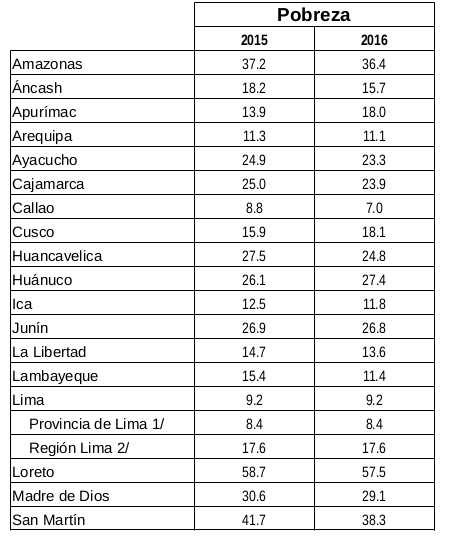
\includegraphics[width=0.4\textwidth]{tabla_1}
  \caption{Datos de pobreza en Per\'u en 2015 y 2016}
  \label{tabla:datos}
\end{figure}

Realizamos el diagrama de dispersi\'on para la pobreza en 2015 vs pobreza
en 2016 y obtenemos los siguientes puntos:\\
\begin{figure}[H]
  \centering
    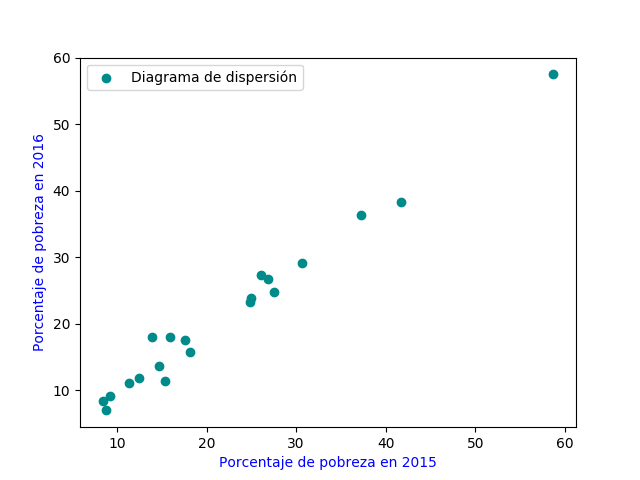
\includegraphics[width=0.55\textwidth]{Figure_1}
  \caption{Diagrama de dispersi\'on}
  \label{figura:dispersion}
\end{figure}

Observamos que los datos pueden tener una relaci\'on lineal para ello debemos 
obtener una ecuaci\'on de la forma:
\begin{center}
  $\hat y=c_0+c_1x$. \textbf{(IV.1)}
\end{center}

De la ecuaci\'on \textbf{(IV.1)} los $x_m$ son los porcentajes de la pobreza en 2015 y 
los $y_m$ son los porcentajes de la pobreza en 2016.

Utilizando el algoritmo en Python obtenemos la siguiente ecuaci\'on:\\
\begin{center}
  $\hat y=0.114103064+0.9608952x$. 
\end{center}
Graficando la ecuaci\'on obtenida:
\begin{figure}[H]
  \centering
    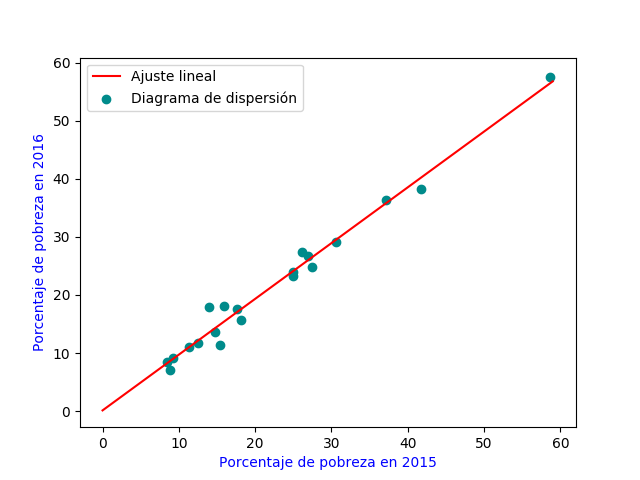
\includegraphics[width=0.55\textwidth]{Figure_2}
  \caption{Ajuste lineal}
  \label{figura:ajuste lineal}
\end{figure}

Ahora analizaremos el resultado de nuestro algoritmo:

\subsection{Calidad de la soluci\'on}
Para comparar nuestro resultado usaremos una librer\'ia llamada sklearn de python que nos da
una ecuaci\'on lineal.
\begin{center}
  $y =  0.11410127044526774 +x 0.96089533$
\end{center}
Tenemos que el error relativo ($E_r$) esta en el siguiente intervalo:
\begin{center}
  $\frac{||R||}{||b||} \frac{1}{Cond(A)} \leq E_r \leq Cond(A)\frac{||R||}{||b||}$
\end{center}
Donde:
\begin{center}
    $R=A\tilde{x}-b$
\end{center}
Realizando los calculos en python tenemos que:
\begin{center}
    $\num{3.44498688e-8} \leq E_r\leq \num{9.40002724e-5}$
\end{center}  
 Con este resultado podemos decir que la soluci\'on es confiable.

\subsection{An\'alisis  de regresi\'on}
Con el fin de determinar la pertinencia de la ecuaci\'on de regresi\'on hallada, es necesario hacer
un an\'alisis de la bondad de ajuste de la recta, demostrar si la relaci\'on es estad\'isticamente
significativa.
Calcularemos las siguientes variables estad\'isticas usando Python:

\subsubsection{El coeficiente de determinaci\'on}

Para la $i$-\'esima observaci\'on de la muestra, la desviaci\'on entre el valor observado de la variable
dependiente y $i$ y el valor estimado de la variable dependiente , se llama $i$-\'esimo residual.
Representa el error que se comete al usar para estimar y $i$ . Tambi\'en se le conoce como la suma
de los cuadrados debidos al error (SSE).
\begin{center}
  $SSE=\sum (y_i - \hat y_i)^2$\\
  $SSE=61.406350402$

\end{center}
El valor de SSE es una medida del error que se comete al usar la ecuaci\'on de regresi\'on para
calcular los valores de la variable dependiente en la muestra.\\
Otro valor de importancia es la medida del error incurrido al usar para estimar y i , llamado suma
total de cuadrados (SST): \\
\begin{center}
  $SST=\sum (y_i - \tilde y)^2$ \\
  $SST=2913.262$

\end{center}
Para saber cu\'anto se desv\'ian los valores de $\hat y_i$medidos en la l\'inea de regresi\'on, de los valores
de $\tilde y$, se calcula otra suma de cuadrados. A esa suma se le llama suma de cuadrados debida a la
regresi\'on, y se representa por SSR.
\begin{center}
  $SSR=\sum (\hat y_i - \tilde y)^2$
  $SSR=2851.854780525$
\end{center}
La relacion entre las medidas es 
\begin{center}
  $SST=SSR+SSE$
\end{center}
La relaci\'on $SSR/SST$, se denomina coeficiente de determinaci\'on y se representa por $r^2$ .
\begin{center}
  $r^2=SSR/SST$\\
  $r^2=0.978921503$
\end{center}
Se puede interpretar a $r^2$ como el porcentaje de la variaci\'on de los valores de 
la variable dependiente que se puede explicar con la ecuaci\'on de regresi\'on.

\subsubsection{Coeficiente de correlaci\'on}

Es la segunda medida que se usa para describir qu\'e tan bien explica una variable a la otra. 
El coeficiente de correlaci\'on de la muestra se denota por $r$ y es la ra\'iz cuadrada del 
coeficiente de determinaci\'on:
\begin{center}
  $r=$(signo de $c_1$)$\sqrt{r}$\\
  $r=0.98940462$
\end{center}
Muestra un coeficiente de correlaci\'on muy alto lo que implica una relaci\'on de dependecia lineal 
fuerte entre los valores de pobreza del 2015 y 2016.
Los coeficientes de determinaci\'on y correlaci\'on no son suficientes para llegar a la conclusi\'on acerca
de si la relaci\'on es estad\'isticamente significativa. Necesitamos realizar una prueba de significancia.\\

\subsubsection{Prueba de significancia}

La ecuaci\'on de regresi\'on lineal simple indica que el valor medio esperado de $y$ es una funci\'on
lineal de $x$ :
\begin{center}
  $E(y)=\beta_0 + \beta_1x$ \\
\end{center}
Si $\beta_1 =0$, entonces $E(y)= \beta_0 $. En este caso el valor medio de $y$ no depende del valor de $x$ y se concluye
que no existe relaci\'on lineal entre las variables. En forma an\'aloga, si el valor de $\beta_1$ no es igual a cero,
se concluye que las dos variables se relacionan. As\'i, para probar si hay alguna relaci\'on importante
de regresi\'on debemos efectuar una prueba de hip\'otesis para determinar si el valor de $\beta$ es cero.
Usaremos la prueba $t$ de Student pero necesitaremos la varianza del error en el modelo de regresi\'on.\\
\textbf{Estimando $\sigma^2$:}\\
La varianza de $\epsilon$, tambi\'en representa la varianza de los valores de respecto a la l\'inea de regresi\'on.
As\'i, la suma de los residuales al cuadrado, $SSE$, es una medida de la variabilidad de las observaciones
reales respecto a la l\'inea de regresi\'on. Cada suma de cuadrados tiene asociado un n\'umero que llamamos grados
de libertad. Se ha demostrado
que $SSE$ tiene $n–2$ grados de libertad, porque se deben estimar dos par\'ametros $\beta_0$ y $\beta_1$
El error cuadrado medio ($^2$ ) es el estimado de $\sigma^2$ .
Se calcula mediante la ecuaci\'on:
\begin{center}
  $s^2=\frac{SSE}{n-2}$ en nuestro caso $n-2=18$
  $3.411463911 $
\end{center}
\textbf{Desviaci\'on est\'andar de la estimaci\'on}\\
El error t\'ipico o desviaci\'on est\'andar del estimado se calcula como la 
ra\'iz cuadrada de la varianza del estimado.
\begin{center}
  $s=\sqrt{\frac{SSE}{n-2}}$\\
  $1.847014865 $
\end{center}

\subsubsection{Realizando la prueba t}

Distribuci\'on muestral de $c_1$:\\
Valor esperado : $E(c_1)=\beta_1$\\
Desviaci\'on est\'andar : $\sigma_{c_1}=\frac{\sigma}{\sqrt{\sum (x_i-\tilde{x})^2}}$\\
Forma de la Distribuci\'on: \textit{Normal}\\
Como no conocemos el valor de $\sigma$ obtenemos una estimaci\'on de $\sigma_{c_1}$, que denotaremos
como $s_{c_1}$.
\begin{center}
  $s_{c_1}=\frac{s}{\sqrt{\sum (x_i-\tilde{x})^2}}$, $s_{c_1}=0.033234007$
\end{center}

Para determinar si la relacion es significativa se basa en el hecho estad\'istico de prueba:
\begin{center}
  $\frac{c_1-\beta_1}{s_{c_1}}$
\end{center}

sigue una distribuci\'on $t$ con $n-2$ grados de libertad. Si la hip\'otesis nula es verdadera, entonces
$\beta_0$ y $t=c_1/s_{c_1}$. Empleando como nivel de significancia $\alpha=0.05$.
$t=\frac{c_1}{S_{b_1}}=28.913010119$\\
En las tablas de distribuci\'on $t$ se encuentra que para $n-2=18$ grados de libertad, $t=2.1009$
da un \'area de $0.025$ en la cola superior.Por lo tanto , el \'area en la cola superior de la
distribuci\'on $t$ correspondiente al valor estad\'istico de prueba $t=28.913010119$  debe ser menor
a $0.025$. Como es una prueba de dos colas, este valor seria $2\cdot (0.025)=0.01$ y se concluye
que el valor-$p$ para $t= 28.913010119$ debe ser menor a $0.01$. Calculando el valor-$p$ con $9$
cifras significativas nos da $0$. Se concluye que $\beta_1$ no es igual a $0$. Esto es suficiente 
evidencia para colcluir que son existe una relaci\'on significativa entre la pobreza del 2015 con la 
pobreza en 2016.

\subsection{Uso de la ecuaci\'on de regresi\'on para estimar y predecir}

Como comprobamos que existe una relaci\'on estad\'isticamente significativa podemos usar 
esa ecuaci\'on para estimar y predecir.
\text{Estimaci\'on de intervalo}\\
Con ese fin, se determinan estimaciones de intervalo. El primer tipo de estimado es el de
intervalo de confianza, que es un estimado del valor medio de $y$para determinado valor de $x$ . El segundo
tipo es el estimado de intervalo de predicci\'on, que se usa cuando deseamos un estimado de intervalo de
valor individual de $y $que corresponda a determinado valor de $x$.

\subsubsection{Estimado del intervalo de confianza del valor medio de y}

Al estimar el porcentaje promedio de pobreza en 2016 de todas las ciudades que en $2015$ mostraron
un \'indice de pobreza de $10.6\%$. El estimado de $E(y_p)$, el valor medio desconocido, es:
\begin{center}
  $\hat y_p=0.114103064+0.9608952(10.6)= 10.299591979$.

\end{center}
Donde $\hat y_p$es el estimado del valor particular de y.
Dado que no se puede esperar que $\hat y_p$sea exactamente igual a $E(y_p)$. Entonces es necesario
considerar la varianza de los estimados basados en la ecuaci\'on de regresi\'on. La f\'ormula para
estimar la desviaci\'on est\'andar de $\hat y_p$dado un valor particular de $x$,$x_p$ es:
\begin{center}
  $S_{\hat y_p}=s\sqrt{\frac{1}{n}+\frac{(x_p-\tilde x)^2}{\sum (x_i-\tilde x)^2}}$.\\
  $S_{\hat y_p}=0.582055397$
\end{center}

La ecuaci\'on general para un estimado del intervalo
de confianza de $E(y_p )$ dado un valor particular $x$ de es:
\begin{center}
  $\hat y_p\pm t_{\alpha/2}\cdot S_{\hat y_p}$  .\\
\end{center}
En donde el coeficiente de confianza es $1-\alpha$ y $t_{\alpha/2}$se basa en una distribuci\'on $t$ con $n-2$ grados de
libertad.

Para determinar un estimado de intervalo de confianza de $95\%$ para el porcentaje promedio
de pobreza en 2016 de todas las ciudades que en 2015 mostraron un \'indice de pobreza de $10.6\%$,
necesitamos el valor de $t$ para $\alpha/2=0.025$ y $n–2= 18$ grados de libertad. As\'i, con $\hat y_p=22,5$ 
 $t_0.025 =2.1009$ $s_{\hat y_p} =0.582055397$, tenemos:
 \begin{center}
  $10.6\pm2.1009\cdot0.582055397$  .\\
  $10.6\pm 1.222840184$ 
\end{center}
Entonces, con una confianza del $95\%$ se puede decir que el porcentaje promedio de pobreza en 2016
de todas las ciudades que en 2015 mostraron un \'indice de pobreza de $10.6\%$ est\'a entre $9.377159816\%$
y $11.822840184\%$.

\subsubsection{Estimado del intervalo de predicci\'on para un valor particular de y}

Para este an\'alisis, se supone que en vez de estimar el valor medio del porcentaje de pobreza, deseamos
estimar el porcentaje de pobreza en 2016 para la regi\'on Tacna con un \'indice de pobreza de $10.6\%$ en 2015.

El estimado para ese valor particular por medio de la ecuaci\'on de regresi\'on es:
\begin{center}
  $\hat y_p=0.114103064+0.9608952(10.6)= 10.299591979$.

\end{center}

Para determinar un estimado del intervalo de predicci\'on debemos determinar primero la
varianza asociada al empleo de $\hat y_p$como estimado de un valor individual de y. Esta varianza est\'a
formada por la suma de dos componentes:
\begin{enumerate}[nosep,label=\arabic*)]
  \item La varianza de los valores individuales de $y$  respecto del promedio cuyo estimado es $s^2$.
  \item La varianza asociada al uso de $\hat y_p$ para estimar $ E(y_p )$ 
  cuyo estimado es $s_{\hat y_p}$.
\end{enumerate}
As\'i, el estimado de la varianza de un valor individual es:
\begin{center}
  $s_{ind}^2=s^2+s_{\hat y_p}$.

\end{center}

Por consiguiente, un estimado de la desviaci\'on est\'andar de un valor un individual de${\hat y_p}$ es:

\begin{center}
  $S_{ind}=s\sqrt{1+\frac{1}{n}+\frac{(x_p-\tilde x)^2}{\sum (x_i-\tilde x)^2}}$.\\
  $S_{ind}=1.93655684$
\end{center}

La ecuaci\'on general para un estimado del intervalo de predicci\'on para un valor individual de $y$ dado
un valor particular de $x$ es:
\begin{center}
  $\hat y_p\pm t_{\alpha/2}\cdot S_{ind}$  .\\
\end{center}

Se tiene que:
\begin{center}
  $10.6\pm2.1009\cdot1.93655684$  .\\
  $10.6\pm 4.068512265$ 
\end{center}

Entonces, con una confianza del $95\%$ se puede decir que el porcentaje de pobreza en 2016 de la 
region Tacna que en 2015 ten\'ia un porcentaje de pobreza de $10.6\%$ est\'a entre $6.531487735\% $
y $14.668512265\%$.

\subsubsection{Estimaci\'on de los par\'ametros del modelo de regresi\'on lineal}

Uno de los conceptos fundamentales sobre el que se ha basado este an\'alisis, es que la ecuaci\'on
de regresi\'on lineal obtenida a partir de los datos de la muestra es un estimado de los par\'ametros
del modelo para la poblaci\'on. Por lo tanto, es posible determinar intervalos de confianza para
los coeficientes de la ecuaci\'on de regresi\'on:
\begin{center}
  $\beta_0=c_0\pm t_{\alpha/2}\cdot s \sqrt{\frac{1}{n}+\frac{\tilde{x}^2}{\sum (x_i-\tilde x)^2}}$  .\\
  $\beta_1=c_1\pm t_{\alpha/2}\frac{s}{\sum (x_i-\tilde x)^2}$ 
\end{center}
De estas f\'ormulas:
\begin{center}
  $\beta_0=0.114103064\pm 1.535177749$  .\\
  $\beta_1=0.960895200 \pm  0.069821325$ 
\end{center}  
Con esta informaci\'on encontramos que la tasa de incremento de la pobreza en
2016 est\'a entre $0.891073675\%$ y $1,030716325\%$ por cada $1\%$ de incremento de la pobreza en 2015 entre una
regi\'on y otra.





\section{Observaciones}
\begin{enumerate}
\item Si incrementamos la cantidad de valores de an\'alisis, es necesario
      paralelizar las transformaciones de Householder y para una
      paralelizaci\'on m\'as sencilla se necesita un nuevo concepto:
      Rotaciones de Givens.
\item Es importante mencionar que los datos encontrados no son actuales por lo
que tal vez no describa perfectamente la tendencia en la actualidad.\\
\item Se puede cometer un error al utilizar el an\'alisis de regresi\'on, 
       y es suponer que un cambio en una variable es “ocasionado” por un cambio en la otra
       variable. Los an\'alisis de regresi\'on y correlaci\'on no pueden, de ninguna manera, 
       determinar la causa y el efecto.
\end{enumerate}



\section{Conclusiones}
\begin{enumerate}
  \item Desde el punto de vista computacional resolver el problema de m\'inimos cuadrados con las
        ecuaciones normales es eficiente, pero esafortunadamente el uso de estas presenta un problema
        de estabilidad num\'erica.

  \item La factorizaci\'on QR usando transformaciones de Householder es un
        gran m\'etodo para realizar ajustes lineales ya que el valor de $E_r$ es bastante peque\~no.

      
  \item El an\'alisis de regresi\'on lineal, como parte de la inferencia estad\'istica, 
  es fundamental para  determinar relaciones de dependencia lineal entre
  variables.
  \item Usando la regresi\'on lineal podemos realizar estimaciones y predicciones dentro de un intervalo
  de confianza deseado.

  \item Con esta herramienta que describe la relaci\'on entre dos varibles podemos hacer ajustes en los
        procesos, tomar decisiones o establecer pol\'iticas.
\end{enumerate}
%\begin{center}
%{\large \bf Agradecimientos}
%\end{center}
%Los autores agradecen a las autoridades de la Facultad de Ciencias de la Universidad Nacional de 
%Ingenier\'{\i}a por su apoyo.
%%\begin{center}
%%{\large \bf Apendice: }
%%\end{center}

\begin{thebibliography}{1}

  \bibitem{Latex}
   L. H\'ector Ju\'arez V.
  \newblock {\em An\'alisis Num\'erico},
  \newblock Setiembre 2008
  
  \bibitem{Latex}
   E. Ward Cheney, David Kincaid
  \newblock {\em Numerical Mathematics and Computing, Seventh Edition},
  \newblock Abril 2012

  \bibitem{Latex}
   Robert Johansson
  \newblock {\em Numerical Python, Second Edition},
  \newblock December 2018


  \bibitem{Latex}
   Wes McKinney
  \newblock {\em Python for Data Analysis, Second Edition},
  \newblock November 2017

  \bibitem{Latex}
   David R.Anderson, Dennis J. Sweeney, Thomas A. Williams
  \newblock {\em Stadistics for Business and Economics, Eleventh Edition},
  \newblock 2010



  
\end{thebibliography}

\end{document}
